%% ------------------------------------------------------------------------- %%
\chapter{Test-Driven Development}
\label{cap:tdd}

Métodos ágeis de desenvolvimento de software focam sempre em constante
feedback, seja ele da equipe em relação ao cliente, ou da equipe em relação a
qualidade (interna e externa) do código produzido \cite{AgileManifesto}. Por
esse motivo, muitas das práticas sugeridas por métodos ágeis tentam aumentar o 
quantidade e a qualidade desse feedback; a ideia da programação pareada, por
exemplo, é dar retorno sobre o código durante sua escrita.

Test-Driven Development (TDD), popularizada por Kent Beck por meio de seu livro
\textit{TDD: By Example} em 2001 \cite{TDDByExample}, é mais uma das práticas
ágeis na qual o foco é dar feedback. TDD tem grande importância durante o ciclo
de desenvolvimento já que, conforme sugerido pelas práticas ágeis, o design de um
software deve emergir a medida que o software cresce. E, para responder
rapidamente a essas alterações, é necessário um constante feedback sobre a
qualidade interna e externa do código.

TDD é uma prática de desenvolvimento de software que se baseia na repetição de
um pequeno ciclo de atividades. Primeiramente, o desenvolvedor deve escrever um
teste que falha. Em seguida, deve fazer esse teste passar, implementando a
funcionalidade desejada. Por fim, deve refatorar o código. Esse ciclo,
exemplificado na figura \ref{fig:red-green-refactor} é também conhecido como 
Vermelho-Verde-Refatora (ou Red-Green-Refactor), já que lembram as cores que o 
desenvolvedor geralmente vê quando faz TDD: o vermelho geralmente significa que
o teste está falhando, e o verde quando o teste foi executado com sucesso.

\begin{figure}
  \centering
  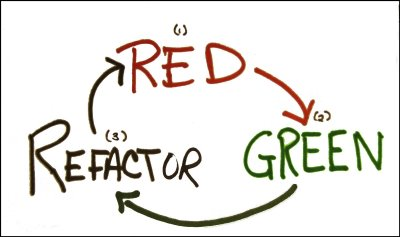
\includegraphics[scale=0.6]{ciclo-tdd}
  \caption{O ciclo Vermelho-Verde-Refatora}
  \label{fig:red-green-refactor}
\end{figure}

A velocidade que a prática dá retorno ao desenvolvedor possibilita que o mesmo
tome decisões sobre o código enquanto o custo de mudança ainda é
baixo. Segundo Vanderburg \cite{vanderburg}, TDD dá feedback em questão de
minutos, e só é inferior a da programação pareada. O gráfico,
baseado no trabalho dele, pode ser visto na Figura
\ref{fig:agile-feedback}.

\begin{figure}
  \centering
  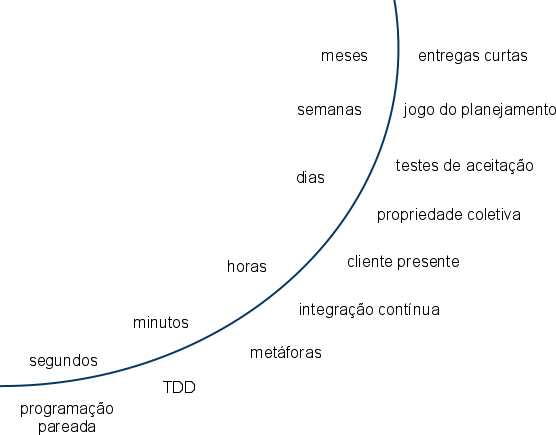
\includegraphics[scale=0.4]{agile-feedback-port}
  \caption{Práticas de XP e Tempo de Feedback (baseado em \cite{vanderburg})}
  \label{fig:agile-feedback}
\end{figure}

%% ------------------------------------------------------------------------- %%
\section{O ciclo}

Um desenvolvedor praticante de TDD escreve os testes antes do código de
produção. Beck define esse ciclo mais especificamente da seguinte maneira
\cite{TDDByExample} e reproduzido na Figura \ref{fig:passos-tdd}:

\begin{enumerate}
	\item Adicione o teste mais simples possível; 
	\item Rode todos os testes e veja o novo teste falhar; 
	\item Escreva o código mais simples que faça o teste passar; 
	\item Rode todos os testes e veja o novo teste passar; 
	\item Refatore para remover duplicação de dados e de código.
\end{enumerate}

Ao iniciar o ciclo, o programador deve escrever o próximo teste mais simples que
ela possa imaginar que falhe; em seguida, ele deve garantir que o teste que ele
escreveu realmente falha; com o teste falhando, o programador deve escrever o
código mais simples que ele possa escrever para fazer o código passar; em
seguida, ele deve checar que o teste que antes falhava, agora passa; por fim, o
programador deve refatorar todo o código duplicado que escreveu.

Simplicidade é algo intrínseco ao processo; o programador deve
buscar sempre escrever o teste mais simples que falhe e escrever o código mais simples
que faça o teste passar. Por fim, a última parte do ciclo é responsável por
tornar o código claro e flexível; nesse momento o programador deve
refatorar o código para remover toda a duplicação de dados ou de código gerada enquanto 
se preocupava em fazer o teste passar da maneira mais simples.

Kent Beck \cite{TDDByExample} afirma que o programador pode tomar
``passos de bebê'' (ou \textit{baby steps}) quando achar necessário. Esses
passos podem ser pequenos a ponto de fazer o programador implementar um método
simplesmente retornando uma constante, quanto maiores, fazendo o programador
implementar o algoritmo final. O programador deve usar sua experiência para
medir o tamanho do passo a ser dado, levando em conta sua confiança e
conhecimento da funcionalidade a ser implementada.

É possível ver que a prática divide o trabalho do desenvolvedor em duas partes.
A primeira se preocupa em escrever um código que funcione (composta pelas
atividades de escrever o teste e fazê-lo passar). Já a segunda parte se preocupa
com um código claro, expressivo e de fácil manutenção (composta pela atividade
de refatoração). Ron Jeffries fez uma famosa afirmação sobre TDD que explica
essa divisão: \textit{``Código claro que funciona''}. Na opinião dele, o programador 
primeiro se preocupa com a parte ``que funciona'', para depois deixar o ``código claro''.

\begin{figure}
  \centering
  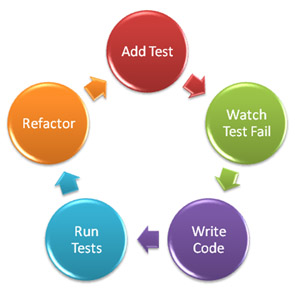
\includegraphics[scale=0.7]{passos-tdd}
  \caption{O ciclo detalhado de TDD.}
  \label{fig:passos-tdd}
\end{figure}

%% ------------------------------------------------------------------------- %%
\section{Benefícios dos testes}

Uma consequência da prática de TDD é a bateria de testes de unidade gerada.
A mesma ajuda o programador a evitar erros de regressão, aonde a implementação de
uma nova funcionalidade quebra uma outra funcionalidade já existente no sistema.
Essa bateria também provê segurança durante as
constantes refatorações de código que são feitas durante o processo de
desenvolvimento, e permite com que ele altere o design e garanta que o
comportamento ainda é o mesmo. 
A cobertura de código coberto pelos testes também tende a ser alta, já que o
desenvolvedor deve sempre escrever um teste antes de implementar uma nova
funcionalidade. Além disso, por ser barato e rápido, a bateria é executada
muitas vezes ao dia, dando feedback constante ao programador.
Dave Astels \cite{astels-tdd} chama essa bateria
de testes de \textit{testes do programador}, já que ele é ferramenta de 
suporte ao trabalho do desenvolvedor.

A simplicidade agregada ao processo também é um dos benefícios da prática de
TDD. Os passos de bebê permitem ao desenvolvedor andar na velocidade que
sentir necessidade, indo mais rápido em partes mais triviais da implementação,
ou mais devagar em trechos mais complexos. Isso leva o desenvolvedor a escrever
códigos mais simples e fáceis de entender.

Em projetos novos, praticantes de TDD afirmam que sentem menos necessidade da
utilização de recursos de depuração de código. A quantidade de código
escrita entre um teste e outro tende a ser pequena, e caso um teste falhe
inesperadamente, o programador pode simplesmente reverter as alterações para a 
versão anterior estável e começar novamente. Essa abordagem pode muitas vezes
ser mais produtiva do que a atividade de depuração 
\cite{janzen-arch-improvement}. Por essas e outras razões, desenvolvedores afirmam 
que são mais produtivos quando praticam TDD. Apesar do custo da escrita do teste
existir, à longo prazo o desenvolvedor gasta menos tempo com depurações ou 
erros de regressão, e com isso tem sua produtividade aumentada
\cite{george-e-williams}.

%% ------------------------------------------------------------------------- %%
\section{TDD e Design}
\label{cap:tdd-e-design}

É comum relacionar TDD à práticas de testes de software. Mas, apesar de ter o
termo ``teste'' no nome, TDD não é uma prática de testes.
Apesar da criação de testes ser algo intrínseco ao processo, TDD é uma prática
que auxilia o desenvolvedor a desenhar classes mais flexíveis, mais coesas e
menos acopladas. Os testes são a ferramenta que o programador utiliza para
validar o design criado. Por esse motivo, muitos se referem a TDD como
\textit{Test-Driven Design}, ou seja, design guiado pelos testes
\cite{tdd-taxonomy}.

Um ponto interessante a ser notado é que nenhum livro sobre TDD \cite{GOOS}
\cite{TDDByExample} \cite{astels-tdd}, discute em momento algum qualquer
prática conhecida da área de testes de software, como análise do valor-limite ou
grafo de causa-efeito \cite{art-of-sw-testing}, o que leva a crer que os
benefícios de TDD não são os mesmos da área de testes.

Muitos autores como Kent Beck \cite{aim-fire}, Dave Astels \cite{astels-tdd} e
Robert Martin \cite{bob-martin} afirmam que TDD é na verdade uma prática de
design \cite{tdd-taxonomy} \cite{aim-fire}.
Na opinião desses autores, a mudança na ordem do ciclo de
desenvolvimento tradicional, apesar de simples, agrega diversos outros
benefícios ao código produzido: simplicidade, foco, melhor design, entre outras.
Ward Cunningham, um dos pioneiros da Programação Extrema resume essa discussão
em uma simples frase: \textit{Test-First programming is not a testing technique}
que, em uma tradução livre, significa \textit{Testar Primeiro não é uma prática 
de testes}.

%% ------------------------------------------------------------------------- %%
\section{Definições incompletas}

Apesar do foco da prática em design, é possível encontrar muitas definições que
não levam isso em conta. Algumas delas levam em consideração apenas a ideia da
inversão da ordem de desenvolvimento, aonde o programador deve primeiro escrever
o teste e depois escrever o código que faça o teste passar.

Um exemplo disso é a definição que pode ser encontrada no livro \textit{JUnit
in Action} \cite{junit-in-action}: \textit{Test-Driven Development é uma
prática de programação que instrui desenvolvedores a escrever código novo
apenas se um teste automatizado estiver falhando, e a eliminar duplicação. O
objetivo de TDD é "código claro que funcione"}.

Apesar de ser correta, ela é incompleta, já que ela não captura um dos pontos
principais da prática, que é feedback no design. Janzen também levanta esse
problema e culpa até o próprio nome da prática, já que ela possui a palavra
``testes'', mas não contém a palavra ``design'' \cite{tdd-really-improve}.

Uma definição mais clara é a de que TDD é a arte de produzir testes
automatizados para código de produção, usando esse processo para guiar o design e a programação.
Para cada pequeno pedaço de funcionalidade, o desenvolvedor deve primeiro
escrever um teste que especifique e valide o que o código irá fazer. O
programador então produz somente o código necessário para fazer esse teste
passar. Então ele refatora (simplifica e clareia) tanto o código de produção
quanto o código de testes \cite{agilealliance-tdd} \cite{tdd-taxonomy}.

Muitos dos artigos utilizados na escrita dessa dissertação apresentam definições
de TDD que não levam em conta seus efeitos no design, e talvez por isso muitas das 
pesquisas em relação à prática avaliam os efeitos de TDD sobre a qualidade 
externa, algo geralmente avaliado em técnicas de testes. Esses estudos são 
explicados com mais detalhes no capítulo \ref{cap:trabalhos-relacionados}.

%% ------------------------------------------------------------------------- %%
\section{Efeitos no Design de Classes}

Na abordagem tradicional, programadores escrevem boa parte do código antes de
testarem. Ao perceberem posteriormente um problema no design, o preço para
corrigir pode ser alto demais. Uma vantagem de escrever os testes antes é
possibilitar que o desenvolvedor tome grande parte das decisões de design
enquanto o custo de mudança ainda é baixo.

O teste é o primeiro cliente da
classe que o programador ainda está por escrever e isso faz com que ele pense
melhor a respeito do comportamento que ele espera da classe. Além disso,
programadores contemplam e decidem também sobre a interface (como nomes de
classes e métodos, tipos de retorno e exceções lançadas) que a classe terá
\cite{janzen-saiedian}.
Além disso, ao escrever o teste antes, o programador é encorajado a escrever um
código que seja facilmente testável. Códigos como esse possuem algumas
características interessantes, como a facilidade para invocar o comportamento
esperado, a não necessidade de pré-condições complicadas e a explicitação de
todas as dependências que a classe possui.

Quanto mais difícil for a escrita do teste, maior a chance da existência de
algum problema de design. Segundo Michael Feathers, existe uma sinergia muito
grande entre uma classe com alta testabilidade e um bom design: se o
programador busca por testabilidade, ele acaba criando um bom design; se o
programador busca por um bom design, ele acaba escrevendo um design mais
testável \cite{feathers-synergy}.

TDD encoraja o programador a escrever componentes fracamente acoplados, de
maneira que eles possam ser testados de maneira isolada, e em um nível maior,
combinados com outros componentes.
Programar voltado para interfaces é uma prática de orientação a objetos há muito
tempo conhecida. Pensar em classes e dar mais foco à maneira com que
elas se relacionam do que com a maneira que elas implementarão determinado
comportamento torna-se mais natural ao praticar TDD \cite{GOOS}. 

%% ------------------------------------------------------------------------- %%
\section{Efeitos na Simplicidade}

TDD sugere que o programador dê sempre pequenos passos (conhecidos pelo termo em
inglês, \textit{baby steps}): deve-se escrever testes sempre para a menor
funcionalidade possível, escrever o código mais simples que faça o teste passar
e fazer sempre apenas uma refatoração por vez \cite{TDDByExample}.

Uma justificativa para tal é que quanto maior o passo que o programador dá, mais
tempo ele leva para concluir esse passo e, consequentemente ele fica mais tempo
sem feedback sobre o código. Além disso, faz com que o programador não crie
soluções mais complexas do que elas precisam ser, tornando o código, à longo
prazo, o mais simples possível.

Uma confusão comum de programadores que experimentam TDD pela primeira vez é a
de que fazer passos de bebê o tempo todo faz com que a produtividade diminua.
De fato, fazer passos de bebê durante todo o ciclo faz com que o tempo de
desenvolvimento aumente, já que muitos desses passos são simples demais e
poderiam ser pulados por um programador mais experiente. 
Mas TDD não força o programador a dar passos de bebê o tempo todo, mas sim
permite que o mesmo dê passos de bebê quando achar necessário
\cite{TDDByExample}. Caso o programador esteja confiante sobre o trecho de
código que está escrevendo naquele momento, ele pode dar um passo maior;  mas
caso ele não esteja tão confiante, a prática permite a ele ir mais devagar e 
dar passos de bebê, obtendo feedback mais rápido sobre o código que está
escrevendo.

O próprio Kent Beck em seu livro afirma que não faz passos tão pequenos o tempo
todo, mas se sente seguro em saber que pode dar passos pequenos quando houver
necessidade.
No exemplo acima, o método \textit{vezes} poderia ser considerado simples por
um programador experiente, que optaria por chegar à mesma solução acima de
maneira mais rápida, tomando passos maiores. Nesse momento, a experiência do
programador deve ditar o ritmo.

O conceito de simplicidade de TDD vai além da implementação de um método; a
simplicidade do design é algo também fundamental. Em modelos tradicionais de
desenvolvimento de software, diagramas de classe são criados para tentar prever
futuras alterações no software, colocando diversos pontos de flexibilização no
modelo. Muitas dessas previsões podem não se concretizar, deixando o design
desnecessariamente complexo.

Equipes ágeis optam por não fazer o chamado \textit{big design up-front (BDUF)},
e deixar que o design emerja ao longo do tempo, mantendo o código o mais claro e
simples possível, e refatorando sempre que há necessidade. Decisões de
design são tomadas com a consciência de que elas serão alteradas no futuro
\cite{is-design-dead}.

Manter o design simples não é tarefa fácil, e TDD sugere que o programador
escreva sempre o código mais simples que atenda a necessidade. Somente se a
necessidade crescer, é que o programador deverá evoluir o design. Uma decisão de
design pode ser mais complicada do que parece e, sem um teste para mostrar isso
rapidamente, o programador dificilmente perceberia o problema \cite{aim-fire}.

Scott Ambler possui uma definição particular sobre como o praticante de TDD lida
com a simplicidade de design. Segundo ele, TDD pode ser definido como
``\textit{TDD = Refatoração + Test-First Design}''. Segundo ele, um programador,
antes de implementar uma nova funcionalidade, deve observar se o design atual
permite que essa funcionalidade seja implementada de maneira clara. Em caso
afirmativo, o programador segue o ciclo, escrevendo um teste que falha e
fazendo-o passar. Mas, em caso negativo, o programador deve refatorar a parte do
design afetado pela nova funcionalidade, de maneira a permitir que ela seja
implementada da maneira mais fácil possível \cite{wambler-tdd}. Perceba que na
visão dele, o programador também deve sempre optar pelo design mais simples, e
somente agregar complexidade se ela for realmente necessária.

%% ------------------------------------------------------------------------- %%
\section{Diferença entre a abordagem tradicional e TDD}
\label{sec:diferencas-tdd-e-tradicional}

Criar classes com baixo acoplamento e alta coesão não é tarefa fácil. Por esse
motivo, é comum que, após algum tempo, os designs percam qualidade e sua
manutenção se torne difícil e, por consequência, cara.
Para evitar esse problema, desenvolvedores constantemente validam a qualidade do
design através de diferentes práticas, como revisões de código, programação
pareada, métricas de código, etc. Praticantes de TDD acreditam que escrever
testes de unidades é útil também para validar a qualidade do design.

Em abordagens tradicionais de desenvolvimento de software, onde o teste é feito
apenas após a funcionalidade ter sido completamenta implementada, o
desenvolvedor acaba por perder o feedback dos testes durante a criação inicial
do design. Ao contrário, o praticante de TDD, por escrever testes
frequentemente, recbee feedback durante todo o processo de escrita do código.

A Figura \ref{fig:tdd-feedback} ilustra dois programadores, usando
abordagens diferentes, escrevendo pequenos pedaços de código para uma
funcionalidade. Praticantes de TDD validam constantemente o design através dos
testes, o que não ocorre com praticantes de abordagens tradicionais, aonde
muitos pequenos pedaços de código são escritos antes dos testes.

\begin{figure}
  \centering
  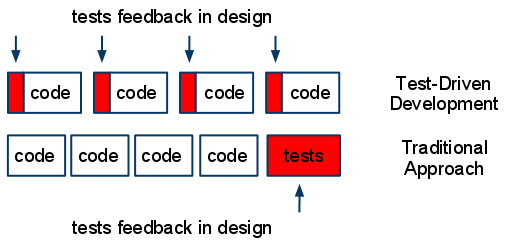
\includegraphics[scale=0.4]{tdd-and-traditional.png}
  \caption{Diferença do feedback dos testes entre praticantes de TDD 
  \\e praticantes de abordagens tradicionais}
  \label{fig:tdd-feedback}
\end{figure}

As informações dadas pelos testes sobre acoplamento e coesão são úteis para
guiar o design. Os testes provêm maneiras de comunicar ao desenvolvedor sobre
possíveis problemas de design. 
